\documentclass[12pt, a4paper, oneside]{report}

\usepackage[T1]{fontenc}
\usepackage[utf8]{inputenc}
\usepackage[spanish]{babel}
\usepackage{hyperref}


% listing for python

\usepackage{listings}
\usepackage{xcolor}

\definecolor{codegreen}{rgb}{0,0.6,0}
\definecolor{codegray}{rgb}{0.5,0.5,0.5}
\definecolor{codepurple}{rgb}{0.58,0,0.82}
\definecolor{backcolour}{rgb}{0.95,0.95,0.92}

\lstdefinestyle{mystyle}{
    backgroundcolor=\color{backcolour},
    commentstyle=\color{codegreen},
    keywordstyle=\color{magenta},
    numberstyle=\tiny\color{codegray},
    stringstyle=\color{codepurple},
    basicstyle=\ttfamily\footnotesize,
    breakatwhitespace=false,
    breaklines=true,
    captionpos=b,
    keepspaces=true,
    numbers=left,
    numbersep=5pt,
    showspaces=false,
    showstringspaces=false,
    showtabs=false,
    tabsize=2
}

\lstset{style=mystyle}

\usepackage{counttexruns}
\usepackage{epigraph}
%%%%%%%%% Preamble file %%%%%%%%%%%%%%
%%%%%%% PACKAGES LOADING %%%%%%%%%%%
%
%
\usepackage[bottom]{footmisc} %keep footnote sticked at the end of the page
%
%
\usepackage{url} %Tratamiento de las urls
\def\UrlBreaks{\do\.\do\@\do\\\do\/\do\!\do\_\do\|\do\;\do\>\do\]%
 \do\)\do\,\do\?\do\'\do+\do\=\do\#\do\&\do\a\do\b\do\c\do\d\do\e%
 \do\f\do\g\do\h\do\i\do\j\do\k\do\l\do\m\do\n\do\o\do\p\do\q\do\r%
 \do\s\do\t\do\u\do\v\do\w\do\x\do\y\do\z\do\A\do\B\do\C\do\D\do\E%
 \do\F\do\G\do\H\do\I\do\J\do\K\do\L\do\M\do\N\do\O\do\P\do\Q\do\R%
 \do\S\do\T\do\U\do\V\do\W\do\X\do\Y\do\Z\do\1\do\2\do\3\do\4\do\5%
 \do\6\do\7\do\8\do\9\do\0}%
%%%%%%%%%%%%%%%%%%%%%%%%%%%%%%%%%%%%
%
%
%%%%%%%% Page Geometry %%%%%%%%%%%%%
\usepackage[top=6cm,bottom=3cm,headheight=4cm, headsep=1cm, footskip=2cm]{geometry}
\usepackage{pdflscape}
%%%%%%%%%%%%%%%%%%%%%%%%%%%%%%%%%%%%
%
%
%%%%%%%%%% Dummy content %%%%%%%%%%%
\usepackage{lipsum}
%%%%%%%%%%%%%%%%%%%%%%%%%%%%%%%%%%%%
%
%
%%%%%%%%% Font & Language %%%%%%%%%%
% XeLaTeX compiler
\usepackage{xltxtra,fontspec,xunicode}
\setsansfont{Verdana}
\usepackage{microtype}
%%%%%%%%%%%%%%%%%%%%%%%%%%%%%%%%%%%%
%
%
%% Enlarge the badboxes tolerances %
\hfuzz=20pt
\vfuzz=20pt
\hbadness=2000
\vbadness=\maxdimen
\emergencystretch 3em%
%
%
%%%%%%%%%%%% Language %%%%%%%%%%%%%
\usepackage[spanish]{babel}
%%%%%%%%%%%%%%%%%%%%%%%%%%%%%%%%%%%%%%
%
%
%%%%%%%%% Floating %%%%%%%%%%%%%%%%%%%
\usepackage{floatrow}
\usepackage{fixmath}
%%%%%%%%%%%%%%%%%%%%%%%%%%%%%%%%%%%%%%
%
%
%%%%%%% Colors & Graphics %%%%%%%%%%%%
\usepackage{amssymb}
\usepackage{soul}
\usepackage{subcaption}
\usepackage[space]{grffile}
\usepackage{tikz}
\usepackage[tikz]{bclogo}
\usetikzlibrary{positioning, arrows, intersections, calc, through, backgrounds, patterns,shapes.geometric}
\usepackage{pgfplots,pgfplotstable}
\usepgfplotslibrary{polar}
\usepackage[american,siunitx]{circuitikz}
\usetikzlibrary{arrows}
\usepackage{lettrine}
\usepackage{amsfonts}
\usepackage{placeins}
\usepackage{longtable}
\usepackage{pgfkeys}
\usepackage{mathtools}
\usetikzlibrary{calc,fadings,decorations.pathreplacing}
%%%%%%%%%%%%%%%%%%%%%%%%%%%%%%%%%%%%%%
%
%
%%%%%%%%%%%%%%% ToC %%%%%%%%%%%%%%%%%%
\setcounter{tocdepth}{2} % Table Of Content depth
%%%%%%%%%%%%%%%%%%%%%%%%%%%%%%%%%%%%%%
%
%
%%%%%%%%%%%%%%% Math %%%%%%%%%%%%%%%%%
\usepackage{amsmath}
\usepackage{amsfonts}
\usepackage{amssymb}
\usepackage{cancel}
\usepackage{units}
\newenvironment{sisalign}{\begin{equation}\left\{\begin{aligned}{}}{\end{aligned}\right.\end{equation}}
\makeatletter
\renewcommand*\env@matrix[1][*\c@MaxMatrixCols c]{%
  \hskip -\arraycolsep
  \let\@ifnextchar\new@ifnextchar
  \array{#1}}
\makeatother %in order to draw vertical lines in bmatrix environment
%%%%%%%%%%%%%%%%%%%%%%%%%%%%%%%%%%%%%%
%
%
%%%%%%%%% Tables Utilities %%%%%%%%%%%
\usepackage{array}
\usepackage{multirow}
\usepackage{booktabs}
\usepackage{longtable}
\usepackage{tabularx}
\usepackage{multicol}
\usepackage{rotating}
\usepackage{tabularx}
\setlength{\tabcolsep}{10pt}
\newcolumntype{L}[1]{>{\raggedright\let\newline\\\arraybackslash\hspace{0pt}}m{#1}}
\newcolumntype{C}[1]{>{\centering\let\newline\\\arraybackslash\hspace{0pt}}m{#1}}
\newcolumntype{R}[1]{>{\raggedleft\let\newline\\\arraybackslash\hspace{0pt}}m{#1}}
%%%%%%%%%%%%%%%%%%%%%%%%%%%%%%%%%%%%%%
%
%
%%%%%%%% Headers Utilities %%%%%%%%%%%
\usepackage{fancyhdr}
\usepackage{lastpage}
%%%%%%%%%%%%%%%%%%%%%%%%%%%%%%%%%%%%%%
%
%
%%%%%%%%%%%%% Codes %%%%%%%%%%%%%%%%%%
\usepackage{listings}  % Source code
\usepackage{moreverb}  % For including source code with tabs
%%%%%%%%%%%%%%%%%%%%%%%%%%%%%%%%%%%%%%
%
%
%%%%%%%%%%%%%% Various %%%%%%%%%%%%%%%
\usepackage{counttexruns}
\usepackage{textcomp}
\usepackage{parskip}
\usepackage{ifthen}
\usepackage{nameref}
\usepackage{enumerate}
\usepackage{placeins}   % Avoid floating frames to be too floating...
\usepackage{eurosym}	% Include euro symbol
\renewcommand{\labelitemi}{$\vartriangleright$}
\renewcommand{\labelitemii}{$\circ$}
%%%%%%%%%%%%%%%%%%%%%%%%%%%%%%%%%%%%%%
%
%
%%%%%%%%%%%% HyperLinks %%%%%%%%%%%%%%
\usepackage[hidelinks]{hyperref}
\hypersetup{%
pdfpagemode={UseOutlines},
bookmarksopen,
pdfstartview={FitH},
plainpages=false
%colorlinks,
%linkcolor={gray},
%citecolor={gray},
%urlcolor={blue}
}
%%%%%%%%%%%%%%%%%%%%%%%%%%%%%%%%%%%%%%
%
%
%%%%%%%%%%%% Bibliography %%%%%%%%%%%%
\usepackage{apacite}
%%%%%%%%%%%%%%%%%%%%%%%%%%%%%%%%%%%%%%
%
%
%%%%%%%%%%%%%%% EPS %%%%%%%%%%%%%%%%%%
\usepackage{epstopdf}
%%%%%%%%%%%%%%%%%%%%%%%%%%%%%%%%%%%%%%
%
%
%%%%%%%% Equations spaces %%%%%%%%%%%%
\let\originalequation\equation
\let\endoriginalequation\endequation
\renewenvironment{equation}
{%
  \originalequation
  \addtolength\abovedisplayshortskip{15pt}
  \addtolength\abovedisplayskip{15pt}
  \addtolength\belowdisplayshortskip{15pt}
  \addtolength\belowdisplayskip{15pt}}
{\endoriginalequation \ignorespacesafterend}
%
\let\originaldisplaymath\displaymath
\let\endoriginaldisplaymath\enddisplaymath
\renewenvironment{displaymath}
{%
  \originaldisplaymath
  \addtolength\abovedisplayshortskip{15pt}
  \addtolength\abovedisplayskip{15pt}
  \addtolength\belowdisplayshortskip{15pt}
  \addtolength\belowdisplayskip{15pt}}
{\endoriginaldisplaymath \ignorespacesafterend}
%%%%%%%%%%%%%%%%%%%%%%%%%%%%%%%%%%%%%%
%
%
%%%%%% Roman Numerals in Text %%%%%%%%
\makeatletter
\newcommand*{\rom}[1]{\expandafter\@slowromancap\romannumeral #1@}
\makeatother
%%%%%%%%%%%%%%%%%%%%%%%%%%%%%%%%%%%%%%
%
%
%% Change Chapter & Section Format %%%
\usepackage{titlesec}
%
\titleformat{\chapter}[display]
{\normalfont\rmfamily\Large\centering}
{\chaptertitlename\ \thechapter}{0pt}{\Huge}
%
\titleformat{\section}
{\normalfont\rmfamily\bfseries}
{\thesection}{1em}{}
%
\titleformat{\subsection}
{\normalfont\rmfamily \slshape}
{\thesubsection}{12pt}{}[]
%
%%%%%%%%%%%%%%%%%%%%%%%%%%%%%%%%%%%%%%
%
%
%%%%% Date format (XX/XX/XXXX) %%%%%%%
\usepackage{datetime}
\newdateformat{dateFMT}
{%
	\twodigit{\THEDAY}/\twodigit{\THEMONTH}/\THEYEAR
}
\newdateformat{monthyeardate}
{%
	\monthname[\THEMONTH] de \THEYEAR
}
%%%%%%%%%%%%%%%%%%%%%%%%%%%%%%%%%%%%%%
%
%
%%%%%% Headers Definition %%%%%%%%%%%%
\headheight=70pt
\fancyheadoffset[L,R]{1cm}
\fancyfootoffset[L,R]{1cm}
\pagestyle{fancy}
\rhead{}
\lhead{}
\chead{\fancyplain{}{%
\renewcommand{\arraystretch}{1.2}
\resizebox{\textwidth}{!}{
\begin{tabular}{l c l}
\toprule
\multirow{3}[2]{*}{
\includegraphics[width=25mm]{Logo/uemc_logo.pdf}} & \multirow{3}{*}{\begin{minipage}{7cm}\begin{center} \textbf{\project} \end{center} \ifthenelse{\equal{\projectshort}{}}{\project}{} \end{minipage}} & Date:\printDate \\
&       & Ed.: \\
&       & Pag.:\thepage\ of \pageref{LastPage}\\ \bottomrule
\end{tabular}}}
}
\renewcommand{\headrulewidth}{0pt}
%%%%%%%%%%%%%%%%%%%%%%%%%%%%%%%%%%%%%%
%
%
%%%%%%%%%%%% COVER PAGE %%%%%%%%%%%%%%
\newlength{\drop}
\newcommand*{\coverPage}
{
	\begingroup%
	\drop=0.1\textheight
	%\vspace*{\drop}
	\vspace*{-2cm}
	\centering
	{
		{\sffamily\fontsize{18}{30}\selectfont%
		\textbf{UNIVERSIDAD EUROPEA\\ \vspace*{10pt}MIGUEL DE CERVANTES}}
		\par
		\vspace*{30pt}
		{\sffamily\fontsize{16}{28}\selectfont%
		\textbf{ESCUELA POLITÉCNICA SUPERIOR}}
		\par
		\vspace*{20pt}
		{\sffamily\fontsize{14}{28}\selectfont%
		\textbf{TITULACIÓN:\\ \vspace*{1pt}MÁSTER UNIVERSITARIO EN GESTIÓN Y ANÁLISIS DE GRANDES VOLÚMENES DE DATOS: BIG DATA}}
		\par
		{
\includegraphics[width=160pt]{Logo/escudo_UEMC.png}}
		\par
		\vspace*{-5pt}
		{\sffamily\fontsize{16}{28}\selectfont%
		\textbf{TRABAJO FIN DE MÁSTER}}
		\par
		\vspace*{30pt}
		{\sffamily\fontsize{22}{34}\selectfont%
		\textbf{\project}}
		\par
		\vspace*{30pt}
		{\sffamily\fontsize{14}{28}\selectfont%
		\textbf{AUTOR}}
		\par
		\vspace*{10pt}
		{\sffamily\fontsize{16}{28}\selectfont%
		\textbf{\authorname}}
		\par
		\vspace*{10pt}
		{\sffamily\fontsize{14}{28}\selectfont%
		\textbf{TUTOR}}
		\par
		\vspace*{10pt}
		{\sffamily\fontsize{16}{28}\selectfont%
		\textbf{\tutoredby}}
		\par
		\vspace*{10pt}
		{\sffamily\fontsize{14}{28}\selectfont%
		\textbf{VALLADOLID, \monthyeardate\today}}
		\par
	}\par
	\endgroup
}
%%%%%%%%%%%%%%%%%%%%%%%%%%%%%%%%%%%%%%
%% ARROW
\newcommand{\arrowTikz}[1]
{
	\begin{tikzpicture}[rotate=#1]
		\coordinate (initPoint)   at (0,0);
		\coordinate (endingPoint) at (0.5,0);
		\draw [line width=1pt,-{Stealth[length=3pt,width=4pt,inset=0.3pt]}](initPoint)--(endingPoint);
	\end{tikzpicture}
}

%% SECTION AND SUBSECTIONS REFERENCE
\newcommand{\refsec}[1]{section~\ref{#1}}
\newcommand{\refsubsec}[1]{subsecsection~\ref{#1}}

%% SUPER & SUB SCRIPT
\newcommand{\superscript}[1]{\ensuremath{^{\textrm{#1}}}}
\newcommand{\subscript}[1]{\ensuremath{_{\textrm{#1}}}}
%% BOLD ITEM
\newcommand\litem[1]{\item{\bfseries #1\enspace} \\}
%% WRITE A VECTOR IN BOLD
\newcommand{\bvec}[1]{\vec{\mathbf{#1}}}
%% PARTIAL DERIVATIVE
\newcommand{\pdv}[2]{\frac{\partial #1}{\partial #2}}
%% BIGO
\DeclareMathAlphabet{\mathpzc}{OT1}{pzc}{m}{it}
\newcommand{\bigO}[1]{$\mathpzc{O}(#1)$}
%% FOR TABLES
\newfloatcommand{capbtabbox}{table}[][\FBwidth]
%% EARTH SPHERE DRAWING
\newcommand\pgfmathsinandcos[3]{%
	\pgfmathsetmacro#1{sin(#3)}%
	\pgfmathsetmacro#2{cos(#3)}%
}
\newcommand\LongitudePlane[3][current plane]{%
	\pgfmathsinandcos\sinEl\cosEl{#2} % elevation
	\pgfmathsinandcos\sint\cost{#3} % azimuth
	\tikzset{#1/.style={cm={\cost,\sint*\sinEl,0,\cosEl,(0,0)}}}
}
\newcommand\LatitudePlane[3][current plane]{%
	\pgfmathsinandcos\sinEl\cosEl{#2} % elevation
	\pgfmathsinandcos\sint\cost{#3} % latitude
	\pgfmathsetmacro\yshift{\cosEl*\sint}
	\tikzset{#1/.style={cm={\cost,0,0,\cost*\sinEl,(0,\yshift)}}} %
}
\newcommand\DrawLongitudeCircle[2][1]{
	\LongitudePlane{\angEl}{#2}
	\tikzset{current plane/.prefix style={scale=#1}}
	% angle of "visibility"
	\pgfmathsetmacro\angVis{atan(sin(#2)*cos(\angEl)/sin(\angEl))} %
	\draw[current plane] (\angVis:1) arc (\angVis:\angVis+180:1);
	\draw[current plane,dashed] (\angVis-180:1) arc (\angVis-180:\angVis:1);
}
\newcommand\DrawLongitudeCircleRed[2][1]{
	\LongitudePlane{\angEl}{#2}
	\tikzset{current plane/.prefix style={scale=#1}}
	% angle of "visibility"
	\pgfmathsetmacro\angVis{atan(sin(#2)*cos(\angEl)/sin(\angEl))} %
	\draw[current plane, color = red] (\angVis:1) arc (\angVis:\angVis+180:1);
	\draw[current plane,dashed, color = red] (\angVis-180:1) arc (\angVis-180:\angVis:1);
}
\newcommand\DrawLatitudeCircle[2][2]{
	\LatitudePlane{\angEl}{#2}
	\tikzset{current plane/.prefix style={scale=#1}}
	\pgfmathsetmacro\sinVis{sin(#2)/cos(#2)*sin(\angEl)/cos(\angEl)}
	% angle of "visibility"
	\pgfmathsetmacro\angVis{asin(min(1,max(\sinVis,-1)))}
	\draw[current plane] (\angVis:1) arc (\angVis:-\angVis-180:1);
	\draw[current plane,dashed] (180-\angVis:1) arc (180-\angVis:\angVis:1);
}
\newcommand\DrawLatitudeCircleRed[2][2]{
	\LatitudePlane{\angEl}{#2}
	\tikzset{current plane/.prefix style={scale=#1}}
	\pgfmathsetmacro\sinVis{sin(#2)/cos(#2)*sin(\angEl)/cos(\angEl)}
	% angle of "visibility"
	\pgfmathsetmacro\angVis{asin(min(1,max(\sinVis,-1)))}
	\draw[current plane,red] (\angVis:1) arc (\angVis:-\angVis-180:1);
	\draw[current plane,dashed,red] (180-\angVis:1) arc (180-\angVis:\angVis:1);
}

%% CAPTION FOR EQUATION SET
\newcounter{equationset}
\newcommand{\equationset}[1]{% \equationset{<caption>}
	\refstepcounter{equationset}% Step counter
	\noindent\makebox[\linewidth]{Ecuaci\'on~\theequationset: #1}}% Print caption
%%%%%%%%%%%%%%%%%%%%%%%%%%%%%%%%%%%%%%
%
%

%%%%%%%%%%%%%% Glossary %%%%%%%%%%%%%%
\usepackage{glossaries}
\makeglossaries
% Definitions and acronyms entries

% \newacronym{uav}{UAV}{Unmanned Aerial Vehicle}
% Reference singular: \gls{uav}   --> UAV
% Reference plural:   \glspl{uav} --> UAVs

% The following definitions will go in the main glossary

% Basics
\newacronym{TFM}{TFM}{Trabajo de Fin de Máster}
\newacronym{UEMC}{UEMC}{Universidad Europea Miguel de Cervantes}
\newacronym{TTF}{TTF}{TrueType Font}
\newacronym{OTF}{OTF}{OpenType Font}
 % Archivo con las entradas del glosario
%%%%%%%%%%%%%%%%%%%%%%%%%%%%%%%%%%%%%%
%
%
%%%%%%%%%%% DOCUMENT DATA %%%%%%%%%%%%
\newcommand{\project}{Title of the project}
\newcommand{\projectshort}{Short Title}
\newcommand{\authorname}{Daniel G.Teba}
\newcommand{\tutoredby}{Miguel Angel Gomez Lopez}
\newcommand{\company}{Universidad Europea Miguel de Cervantes}
\newcommand{\doctype}{Draft} %or draft
\newcommand{\revision}{\thecounttexruns}
\newcommand{\printDate}{\dateFMT\today}
%%%%%%%%%%%%%%%%%%%%%%%%%%%%%%%%%%%%%%
%
%
%%%%%%%%%%% PDF METADATA %%%%%%%%%%%%%
\hypersetup{pdftitle={\project},
	pdfauthor={Daniel G.Teba},
	pdfsubject={\project},
	pdfkeywords={\company}
}
%%%%%%%%%%%%%%%%%%%%%%%%%%%%%%%%%%%%%%
%
%
%%%%%%%%% DRAFt TWATERMARK %%%%%%%%%%%
\ifthenelse{\equal{\doctype}{Draft} \or \equal{\doctype}{draft}}
{
	\usepackage[angle=60,
				color=black!40,
				scale=5]{background}
	\usepackage{graphicx}}{}
	\backgroundsetup{contents={DRAFT \printDate}}
%%%%%%%%%%%%%%%%%%%%%%%%%%%%%%%%%%%%%%
%
%
%%%%%%%%%%%% DOCUMENT %%%%%%%%%%%%%%%%
\begin{document}
	%\renewcommand{\abstractname}{Abstract}
	%\renewcommand{\appendixname}{Ap\'endices}
	%\renewcommand{\bibname}{Bibliograf\'ia}
	%\renewcommand{\chaptername}{Cap\'itulo]
	\renewcommand{\contentsname}{Índice de contenidos}
	\renewcommand{\figurename}{Figura}
	\renewcommand{\listfigurename}{Índice de figuras}
	\renewcommand{\listtablename}{Índice de tablas}
	\renewcommand{\tablename}{Tabla}

	\setcounter{counttexruns}{5}
	\thispagestyle{empty}
	\coverPage
	\thispagestyle{empty}

	\clearpage
	\tableofcontents
	\listoffigures
	\listoftables
	\clearpage

	\chapter{Objetivos del trabajo}

Dados unos datos experimentales provenientes de una nariz electrónica,
\textbf{insertar aquí enlace UCI data} se desea hacer un estudio de la viabilidad de
clasificar correctamente de qué gas se trata,
e intentar dar una estimación de la concentración de dicho gas.

Los datos provienen de cada medición de un gas con 16 sensores.
De esta forma, cada medición genera 16 series temporales, de las cuales de cada una se
han extraido 8 \emph{features}. Esto hace un total de 128 componentes para cada medición.
Para cada medición es conocido el gas que se ha ensayado y su nivel de concentración.

Con este tipo de información, se va a estudiar los resultados que pueden ofrecer las redes neuronales
para resolver este problema.

En el caso que nos ocupa, los sensores derivan a
lo largo del tiempo, lo cual implica que para el mismo gas, con la misma concentración, las series temporales obtenidas
en un mes dado podrían ser diferentes a las realizadas con las mismas condiciones meses después.

En este trabajo se tomará como primera aproximación dividir la tarea de clasificación y la tarea de estimación.

Para la tarea de clasificación, se probarán las siguientes configuraciones, de más simple a más compleja:

\begin{itemize}
    \item Perceptron
    \item \textbf{Long short-term memory \glossary{LSTM} Neural net}
\end{itemize}

Una vez conseguida la tarea de clasificación, se usará otra red neuronal para determinar, si es posible,
la concentración del gas.

En este trabajo se utilizará Keras y TensorFlow para el diseño de las redes neuronales, en el entorno Python.


	\clearpage

	\chapter{Ánalisis de la situación}

El principal objetivo del dataset de Gas Drift de UCI es proporcionar un bechmark donde probar las diferentes soluciones
y algoritmos para afrontar el problema de la deriva de sensores de gas, también conocidos como narices electrónicas.

En la Figure \ref{fig:sensorphoto} \cite{Zhao2019} podemos ver la disposición del sistema de adquisición para construir el dataset que finalmente está disponible en UCI.

El gas pasa por la placa de adquisición, donde las señales temporales generadas por cada sensor (Figura \ref{fig:sensor_response}) se descomponen en dos componentes de continua y 6 componentes de transitorio, 3 caracterizando la entrada del gas, y 3 caracterizando la salida. En la Figura \ref{fig:tabfeatures} se resumen estas carateristicas. Para más detalle del significado de las componentes consultar \cite{Vergara2011}

Por tanto el dataset proporcionado caracteriza a cada gas con 128 componentes obtenidas de los diferentes sensores, 1 componente que especifica la concentración presente de ese gas en la medición, y el batch al que pertenece la medición, es decir,
en qué meses se realizó. En total tendríamos 2 variables objetivo (gas y concentración), 128 características, y una componente temporal (batch id).

Esto presenta un reto para entrenar un algoritmo de clasificación, por varios motivos:
\begin{itemize}
\item Para un mismo gas, los sensores capturaran diferentes respuestas para diferentes concentraciones
\item Una medición de un gas a una concentración dada, no será igual en los primeros meses de medición que en los últimos, debido a la deriva del sensor.
\item Se han usado 4 tipos de sensores, y dentro de cada tipo se usaron 4 calibraciones diferentes \cite{Zhao2019} por lo que podría darse la situación de que algún sensor no sea capaz de detectar el paso del gas, o se vea saturado, dando una medición no valida para clasificar.
\end{itemize}

En este trabajo primero comprobaremos que
\begin{itemize}
	\item Existe esta deriva de los sensores. Comparación de la misma señal a lo largo de los meses.
	\item Esta deriva afecta a los modelos de clasificación. Modelo de clasificación muy sencillo con una red neuronal secuencial.
	\item Existe correlación entre las mediciones de los 16 sensores, ya que se trata de 16 mediciones del mismo fenómeno. Es más, las 8 componentes la descomposición propuesta de la señal, no son independientes entre sí.
\end{itemize}

\begin{figure}
	\centering
	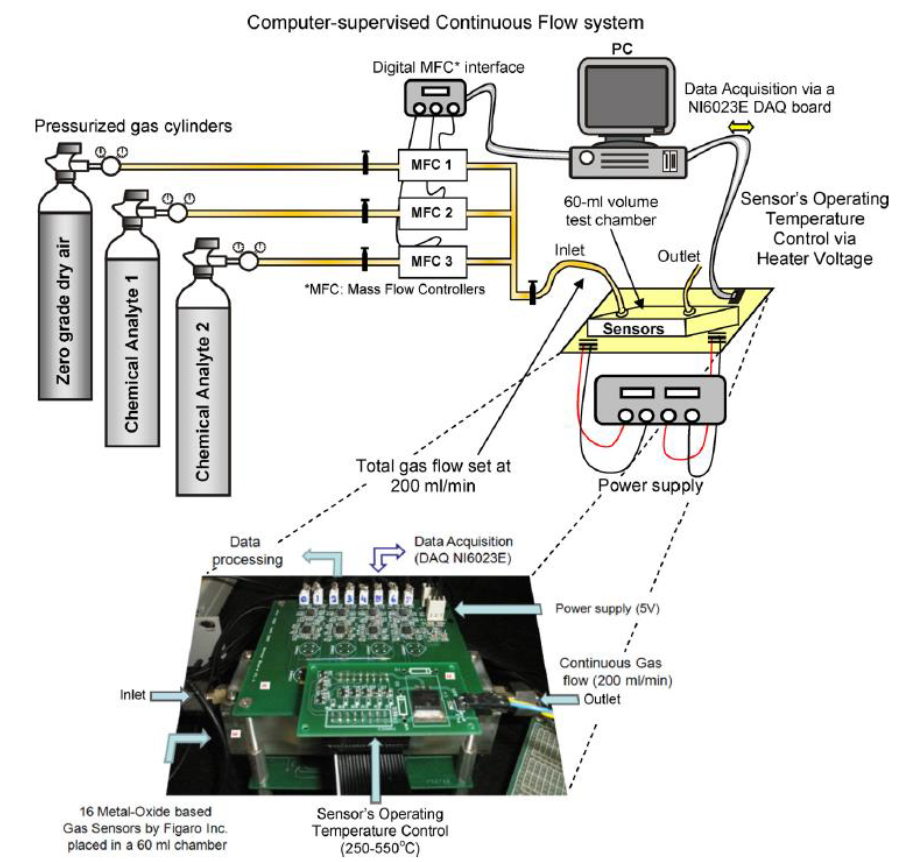
\includegraphics[width=0.95\linewidth]{../py_imgs/sensor_photo}
	\caption[Esquema de sistema de adquisición de datos]{Esquema del sistema de adquisición, donde pueden verse los 16 sensores de gas Figaro.}
	\label{fig:sensorphoto}
\end{figure}

\begin{figure}
	\centering
	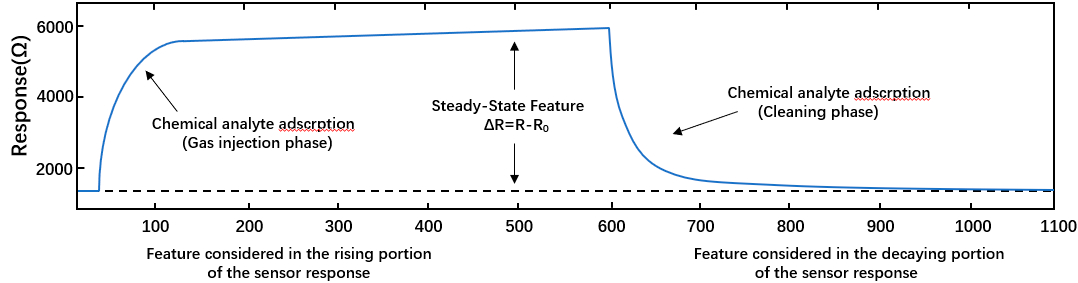
\includegraphics[width=0.95\linewidth]{../py_imgs/sensor_response}
	\caption[Respuesta del sensor]{Información típica de la respuesta del sensor. Respuesta típica de una sustancia química a base de óxido metálico sensor a 30ppmv de acetaldehído. La curva muestra las tres fases de una medición: línea de base medición (realizada con aire puro), medición del gas de prueba (cuando se inyecta el analito químico, en forma de gas, a la cámara de prueba) y fase de recuperación (durante la cual el sensor se expone nuevamente a aire puro; el tiempo de recuperación suele ser mucho más largo que la inyección de gas\protect\cite{Vergara2011}}
	\label{fig:sensor_response}
\end{figure}

\begin{figure}
	\centering
	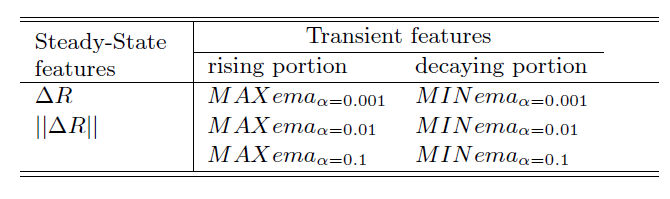
\includegraphics[width=0.95\linewidth]{../py_imgs/tab_features}
	\caption[Descomposición de las señales temporales]{Descripción de la descomposición de las señales temporales generadas por los sensores. Más información en \protect\cite{Vergara2011}}
	\label{fig:tabfeatures}
\end{figure}

	\clearpage

	\chapter{Obtención, procesado y almacenamiento de los datos}


%Obtencion
Los datos provienen del artículo  Chemical gas sensor drift compensation using classifier ensembles \cite{GasData},

donde el objetivo era tratar de detectar el drift (la deriva) de los sensores a lo largo de los meses, y poder calibrarlos
utilizando el minimo numero de experimentos posibles. Es decir, de la forma más rápida y eficiente posible.
(ver \cite{GasData})

Los datos estan disponibles para su descarga desde
\href{https://archive.ics.uci.edu/ml//datasets/Gas+Sensor+Array+Drift+Dataset#}{UCI data repository}.
en 10 archivos formato \emph{.dat}.

Cada lote cuenta con una estructura de 129 columnas, donde la primera nos informa del gas y la concentración,
y el resto es la información obtenida del sensor.

El primer paso que se va a realizar es, dada las 128 componentes X,
averiguar a qué tipo de gas pertenece la medición.

Una vez la red es capaz de inferir correctamente de qué gas se trata,
alimentaremos otra red cuya función
sea averiguar la concentración del mismo.

\subsection{Procesado}

La lectura de los archivos  \emph{.dat} se ha realizado utilizando
el código adjunto en Apendices  \ref{LoadUciData}


\subsection{Exploratory Data Analysis}

Los datos se nos presentan en 10 lotes, correspondientes a experimentos a lo largo de tres años, donde se ensayaron
6 diferentes gases a diferentes concentraciones.

\begin{table}[h!]
\begin{tabular}{|l|l|}
\hline
Batch ID & Month IDs                   \\ \hline
Batch 1  & Months 1 and 2              \\
Batch 2  & Months 3, 4, 8, 9 and 10    \\
Batch 3  & Months 11, 12, and 13       \\
Batch 4  & Months 14 and 15            \\
Batch 5  & Month 16                    \\
Batch 6  & Months 17, 18, 19, and 20   \\
Batch 7  & Month 21                    \\
Batch 8  & Months 22 and 23            \\
Batch 9  & Months 24 and 30            \\
Batch 10 & Month 36                    \\
\end{tabular}
    \caption{ Distribución de los lotes a lo largo del tiempo.}
\end{table}

Los gases que se estudiaron son los siguientes:
\begin{enumerate}
    \item Ethanol
    \item Ethylene
    \item Ammonia
    \item Acetaldehyde
    \item Acetone
    \item Toluene
\end{enumerate}

Los lotes contienen una cantidad de muestras desigual, ni los 6 gases de estudio están presentes en todos los lotes.

La tabla \ref{Tab: Numero de Gases por cada Batch} muestra el numero de ensayos para cada gas.

\begin{table}
    \centering
    \begin{tabular}{|l|l|l|l|l|l|l|l|}
    \hline
         & Batch ID & 1 & 2 & 3 & 4 & 5 & 6 \\ \hline
        1 & 90   & 98  & 83  & 30  & 70  & 74 &  \\ \hline
        2 & 164  & 334 & 100 & 109 & 532 & 5   &  \\ \hline
        3 & 365  & 490 & 216 & 240 & 275 & 0   &  \\ \hline
        4 & 64   & 43  & 12  & 30  & 12  & 0   &  \\ \hline
        5 & 28   & 40  & 20  & 46  & 63  & 0   &  \\ \hline
        6 & 514  & 574 & 110 & 29  & 606 & 467 &  \\ \hline
        7 & 649  & 662 & 360 & 744 & 630 & 568 &  \\ \hline
        8 & 30   & 30  & 40  & 33  & 143 & 18  &  \\ \hline
        9 & 61   & 55  & 100 & 75  & 78  & 101 &  \\ \hline
        10 & 600 & 600 & 600 & 600 & 600 & 600 &  \\ \hline
    \end{tabular}
    \label{Tab: Numero de Gases por cada Batch}
\end{table}

En la Tabla\ref{Tab: Numero de Gases por cada Batch} podemos ver que el número de muestras en cada lote
es desigual. En los lotes 3, 4 y 5 el gas 6 no está presente. A la hora de crear un dataset de entrenamiento,
convendria generar un lote donde haya un numero equitativo de muestras de todos los gases,
y si las mediciones no son distantes en el tiempo podremos ver el efecto de la deriva si el algorimo entrenado con
los primeros lotes falla para cada vez más conforme nos alejamos en el tiempo.

La Figura \ref{fig: gasBatchCount} muestra la cantidad de gases ensayados por lote, mientras que
la Figura\ref{fig: gasCount} muestra el numero de mediciones totales sobre cada gas.

\begin{figure}[ht!]
	\centering
	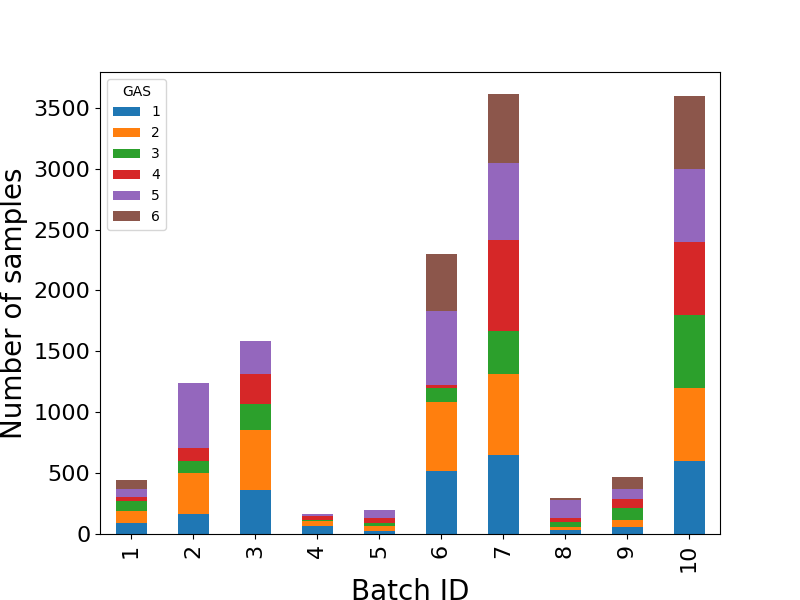
\includegraphics[width=\columnwidth]{../py_imgs/Step0_Count_Batch_Gas.png}
	\caption{Número de muestras de gas por Batch}
	\label{fig: gasBatchCount}
\end{figure}

\begin{figure}[ht!]
	\centering
	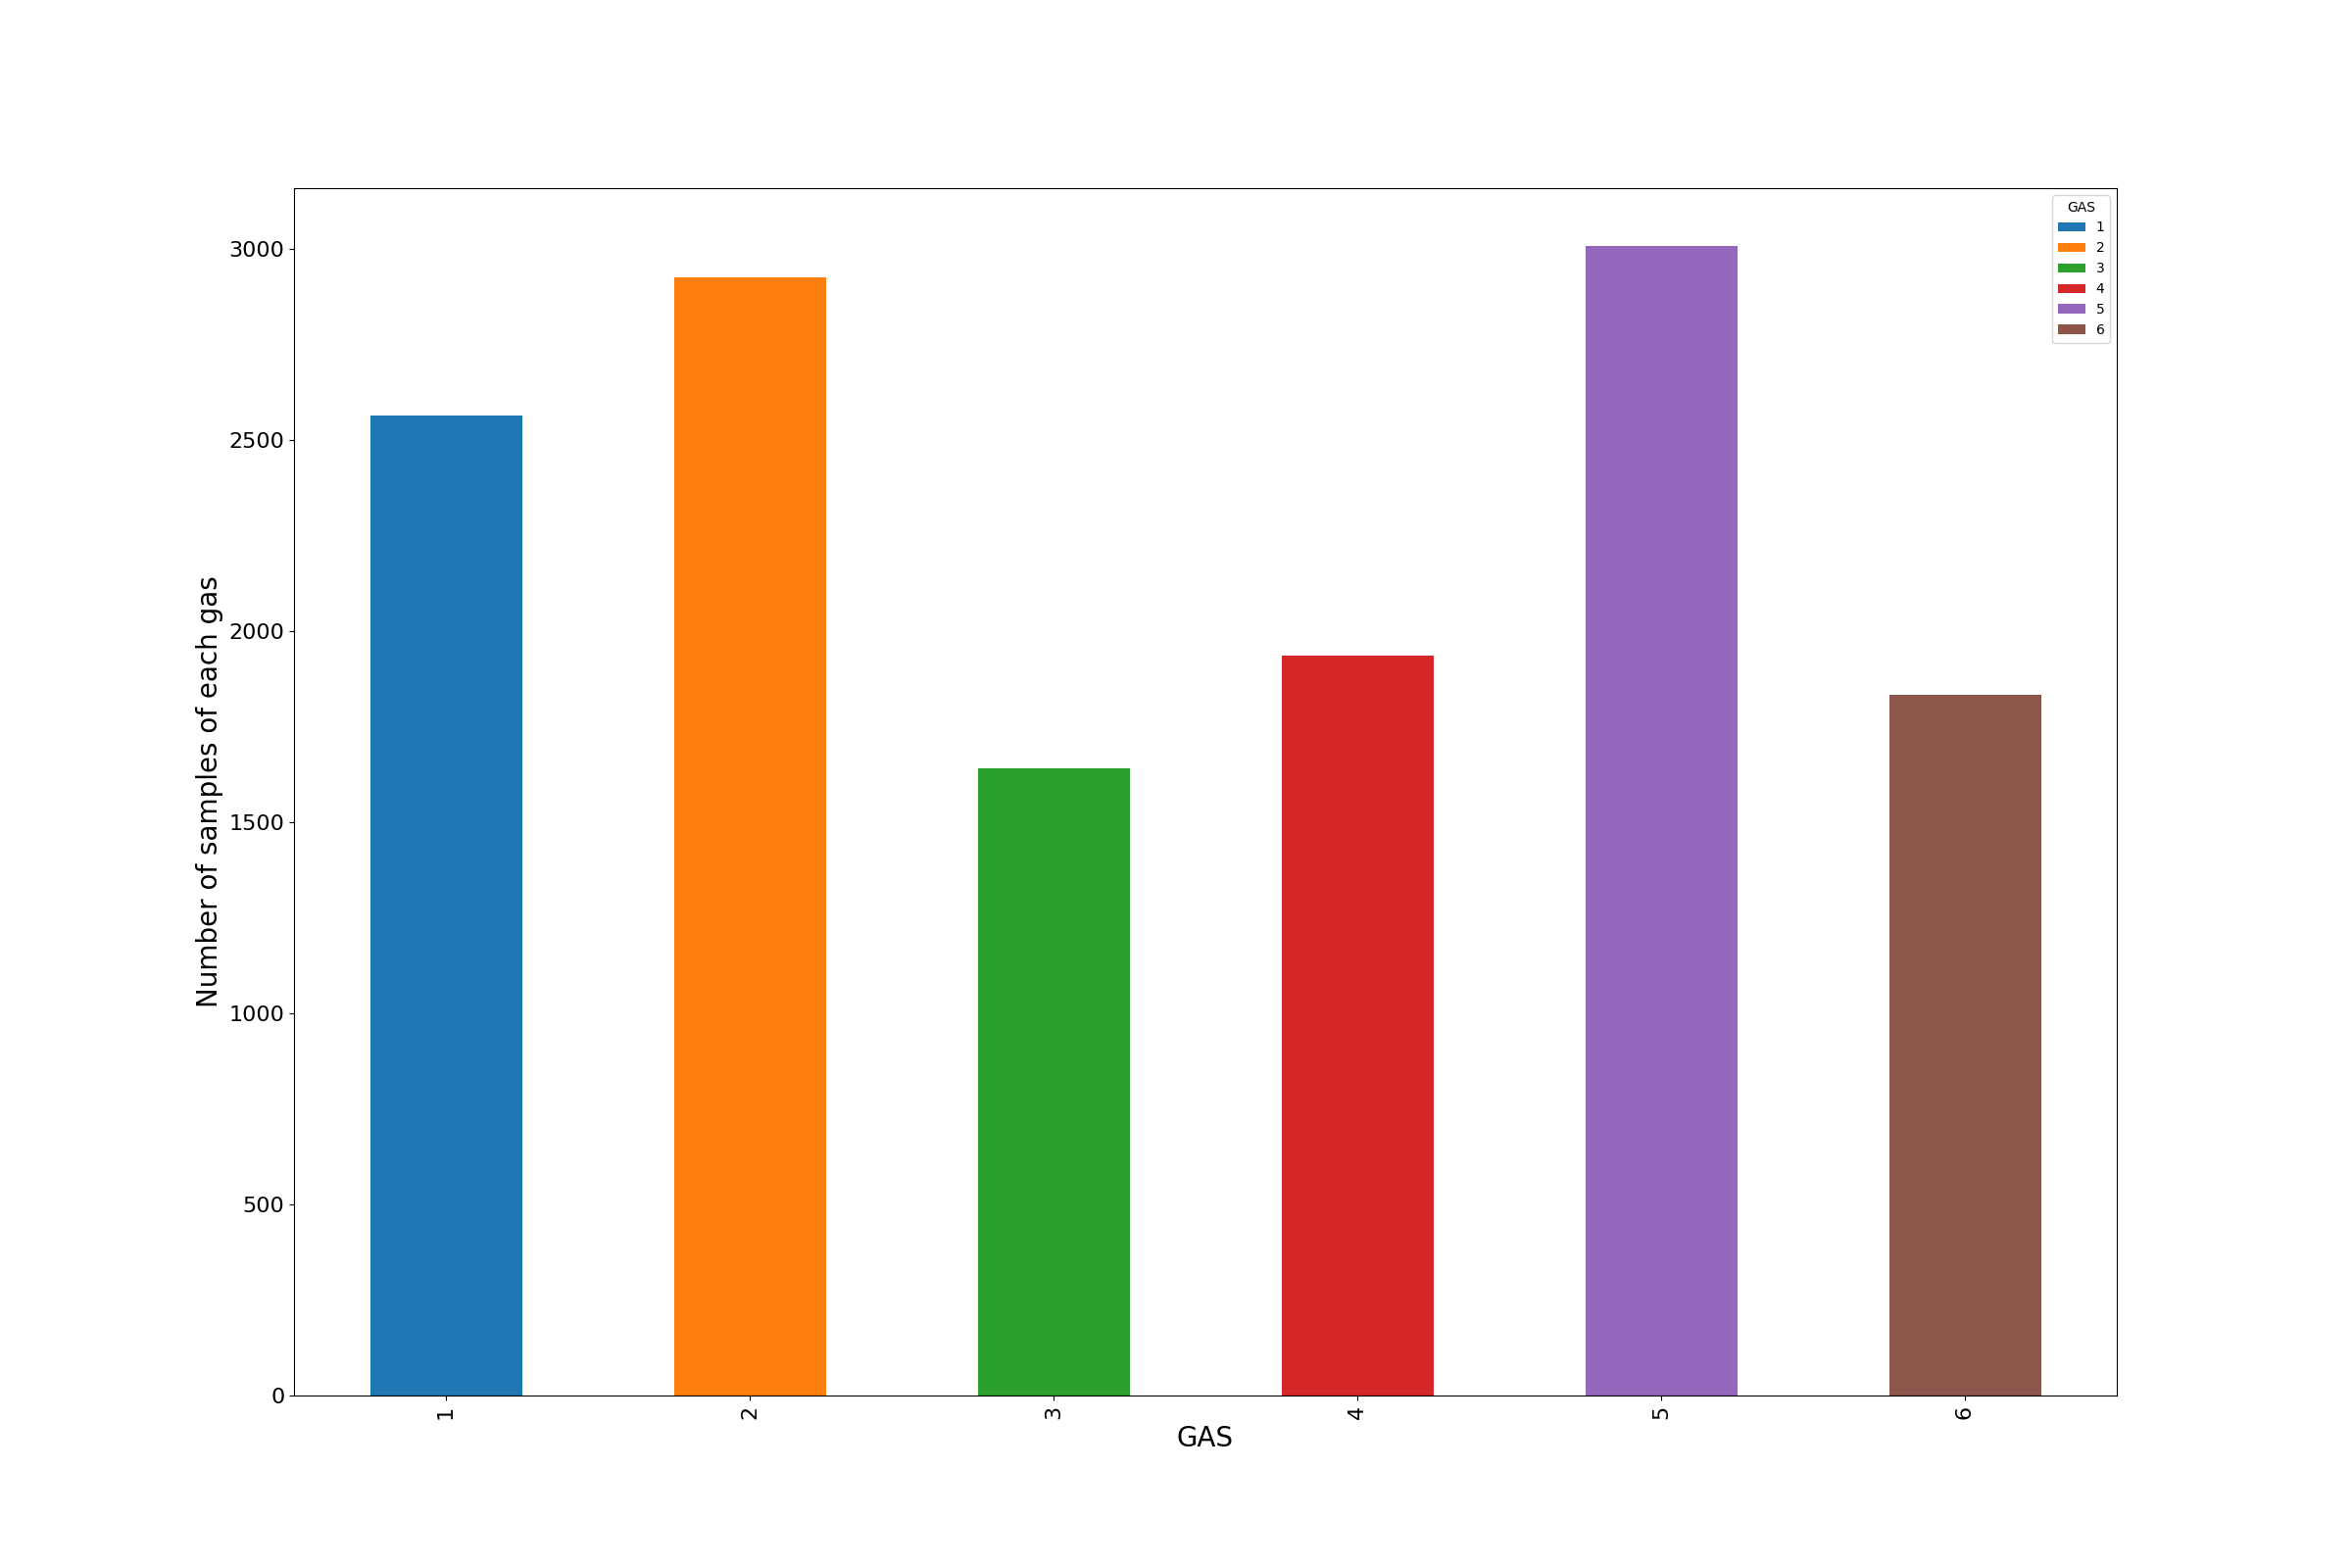
\includegraphics[width=\columnwidth]{../py_imgs/Step0_Count_Gas.png}
	\caption{Número de muestras de cada gas en total}
	\label{fig: gasCount}
\end{figure}

Si observamos los rangos de concentración para cada gas, han sido también diferentes.

\begin{table}
    \centering
    \begin{tabular}{|l|l|l|l|l|l|}
    \hline
         & GAS & Minimo & Máximo & Media & StdDesv \\ \hline
        1 & 2.5 & 600 & 114.95 & 86.64 &  \\ \hline
        2 & 2.5 & 300 & 116.1 & 79.89 &  \\ \hline
        3 & 2.5 & 1000 & 323.55 & 272.02 &  \\ \hline
        4 & 2.5 & 300 & 126.32 & 76.71 &  \\ \hline
        5 & 10 & 1000 & 228.57 & 217.38 &  \\ \hline
        6 & 1 & 230 & 47.66 & 32.58 &  \\ \hline
    \end{tabular}
\end{table}

Esta información es necesario tenerla en cuenta a la hora de entrenar nuestro modelo, ya que
si el rango de variación de los datos es dispar, será recomendable normalizar.





	\clearpage

	\chapter{Diseño e implementación de los modelos o técnicas necesarias}


\section{Modelo secuencial}
En este capítulo se ah diseñado una red neuronal muy sencilla, con itención de observar los efectos que el drift puede tener en el accuracy y el loss del modelo. El esquema de la red neuronal se presenta en la tabla \ref{tab:esquemaRNN}

\begin{table}
	\centering
	\begin{tabular}{|l l l|}
		\toprule
		Model: "sequential"  & &   \\ \midrule 
		Layer (type)         &        Output Shape   &         Param  \\ \hline
		flatten (Flatten)    &        (None, 128)    &         0      \\ \hline
		dense (Dense)        &        (None, 32)     &         4128   \\ \hline
		dense\_1 (Dense)     &         (None, 32)    &         1056  \\ \hline
		dense\_2 (Dense)     &         (None, 6)     &         198   \\ \hline
		Total params: 5,382  &                       &     \\ \hline
		Trainable params: 5,382 & & \\ \hline
		Non-trainable params: 0 & & \\ \bottomrule
	\end{tabular}
\caption[Modelo de red neuronal secuencial]{Modelo de red neuronal secuencial \label{tab:esquemaRNN}}
\end{table}

\subsection{Modelo simplificado}

Primero, modelo más simple posible. Los datos de entrenamiento serán las mediciones de 1 sensor y como valores objetivo tomamos pares gases-concentración . Es decir, reducimos las mediciones a 6 parejas gas-concentración únicas tomadas por un único sensor.

Reducimos así las variables de estudio, y podemos ver el efecto del drift en las mediciones de un gas dado. Utilizando todos los datos, división entre entrenamiento y validación al 70/30, obtenemos la matriz de confusión de la Figura\ref{fig:confmatrixmodelsimple}

\begin{figure}
	\centering
	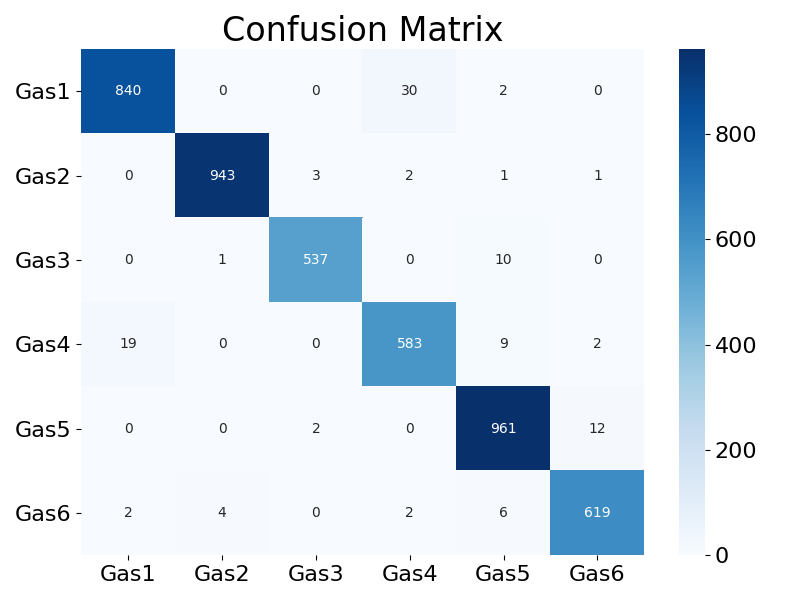
\includegraphics[width=0.7\linewidth]{../py_imgs/ConfMatrix_ModelSimple}
	\caption{Matriz de confusión del modelo utilizando todas las mediciones, entrenando al 70/30. Muy buenos resultados.}
	\label{fig:confmatrixmodelsimple}
\end{figure}

Sabemos que nuestro modelo a podido aprender a diferenciar entre los gases, pero no es realmente útil, ya que el modelo está aprendiendo cómo es un gas tanto en el primer mes de mediciones como en el último. Es decir, este modelo daría malos resultados si probamos con nuevas mediciones.

\subsection{Modelo completo}


Si este mismo modelo lo entrenamos con todos los datos disponibles de los sensores, el primer batch, y medimos el accuracy y el loss frente a los siguientes batch, obtenemos las Figuras\ref{fig:EvoModelSimpleBatch}. Se observa claramente cómo tanto el accuracy decae conformo intentamos predecir valores más lejanos. 

\begin{figure}
	\centering
	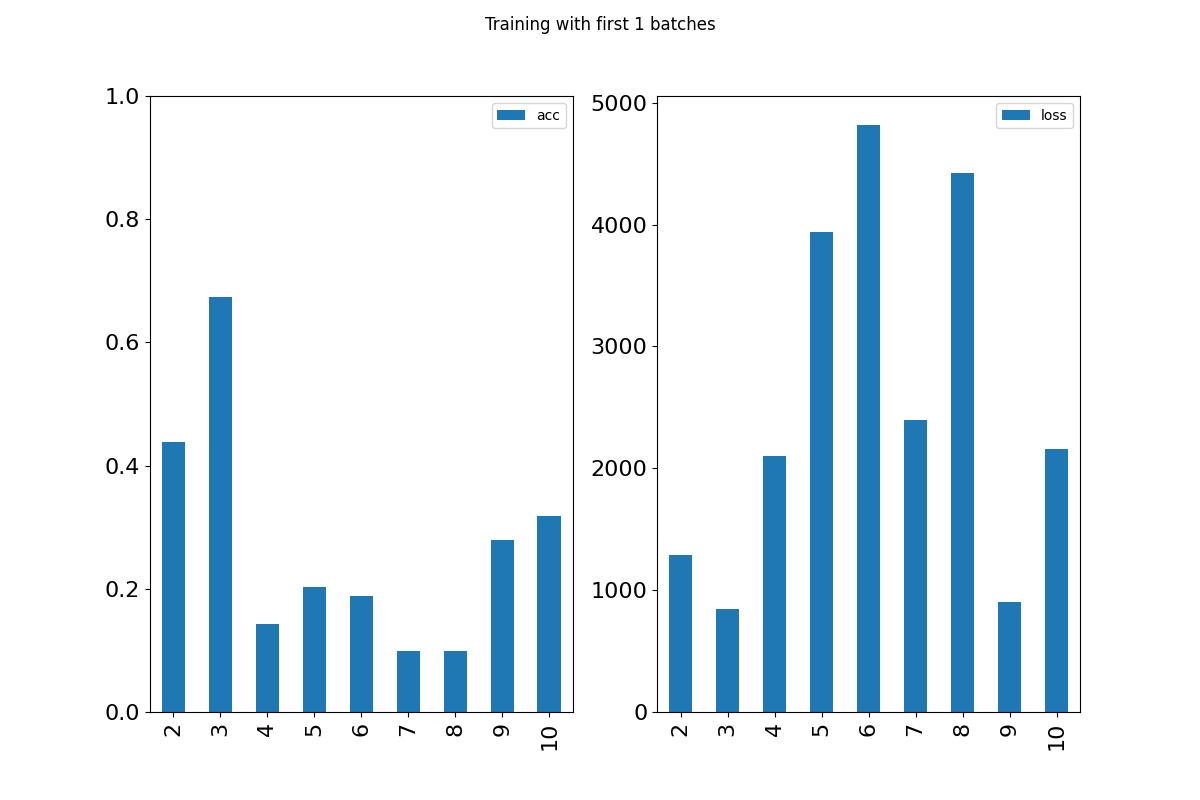
\includegraphics[width=0.45\linewidth]{../py_imgs/Step1_NBATCH_1_acc_loss}
	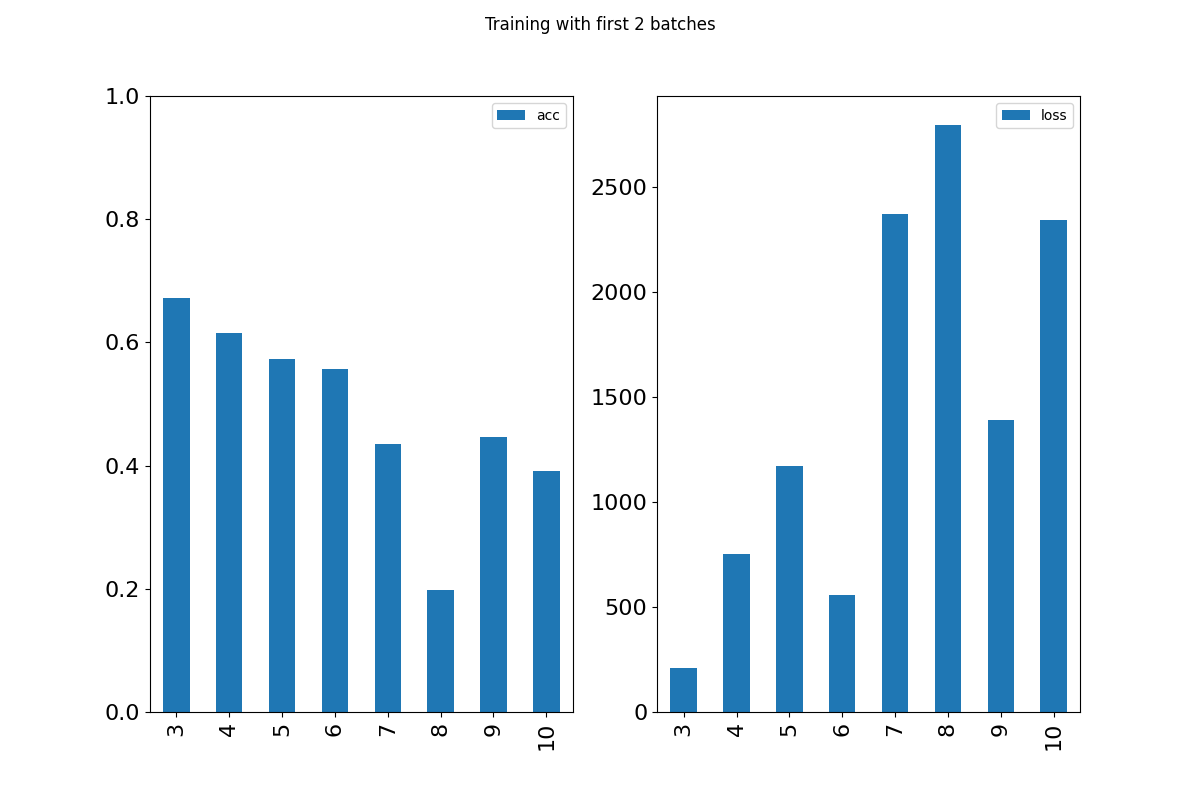
\includegraphics[width=0.45\linewidth]{../py_imgs/Step1_NBATCH_2_acc_loss}
	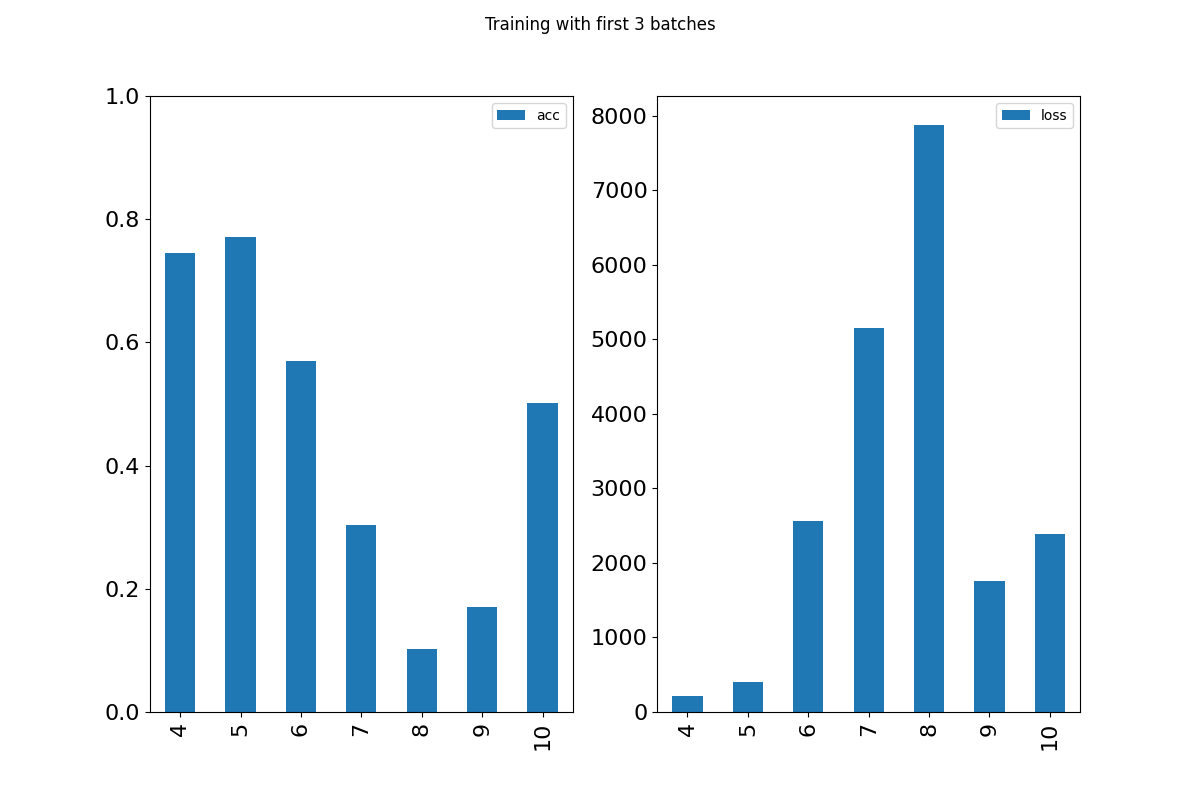
\includegraphics[width=0.45\linewidth]{../py_imgs/Step1_NBATCH_3_acc_loss}
	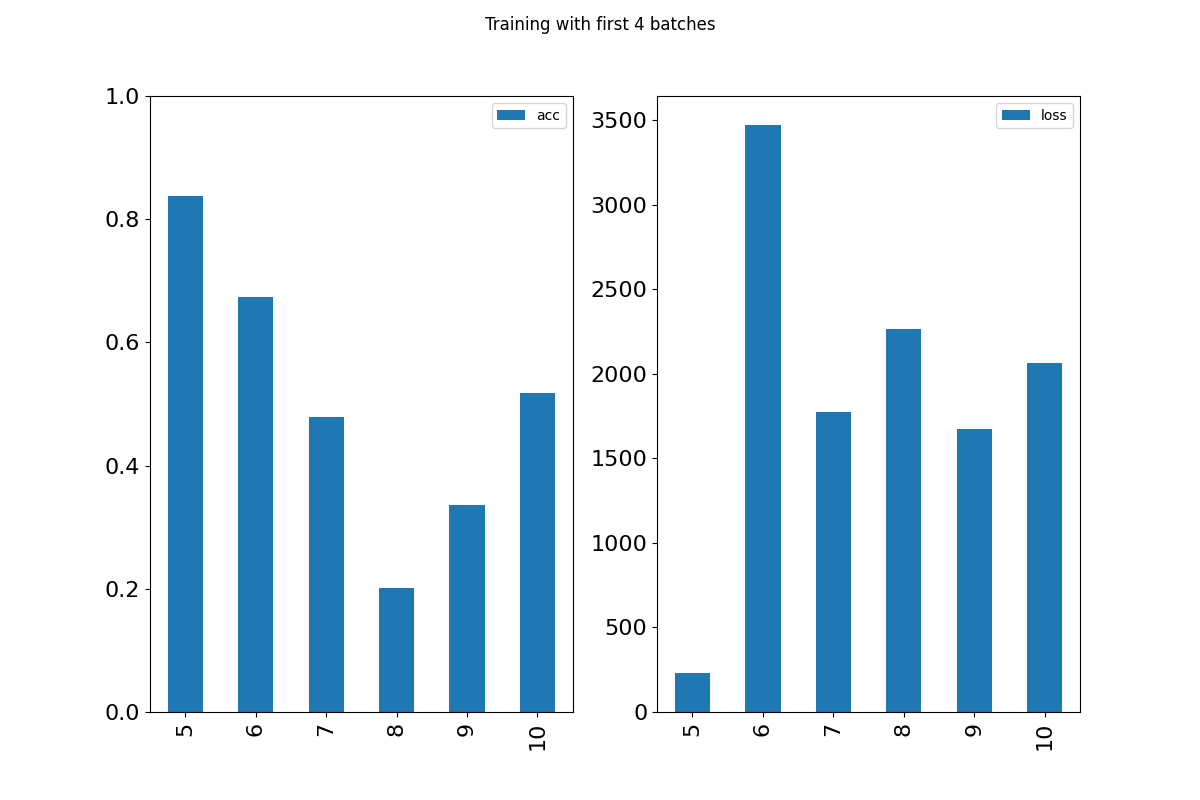
\includegraphics[width=0.45\linewidth]{../py_imgs/Step1_NBATCH_4_acc_loss}
	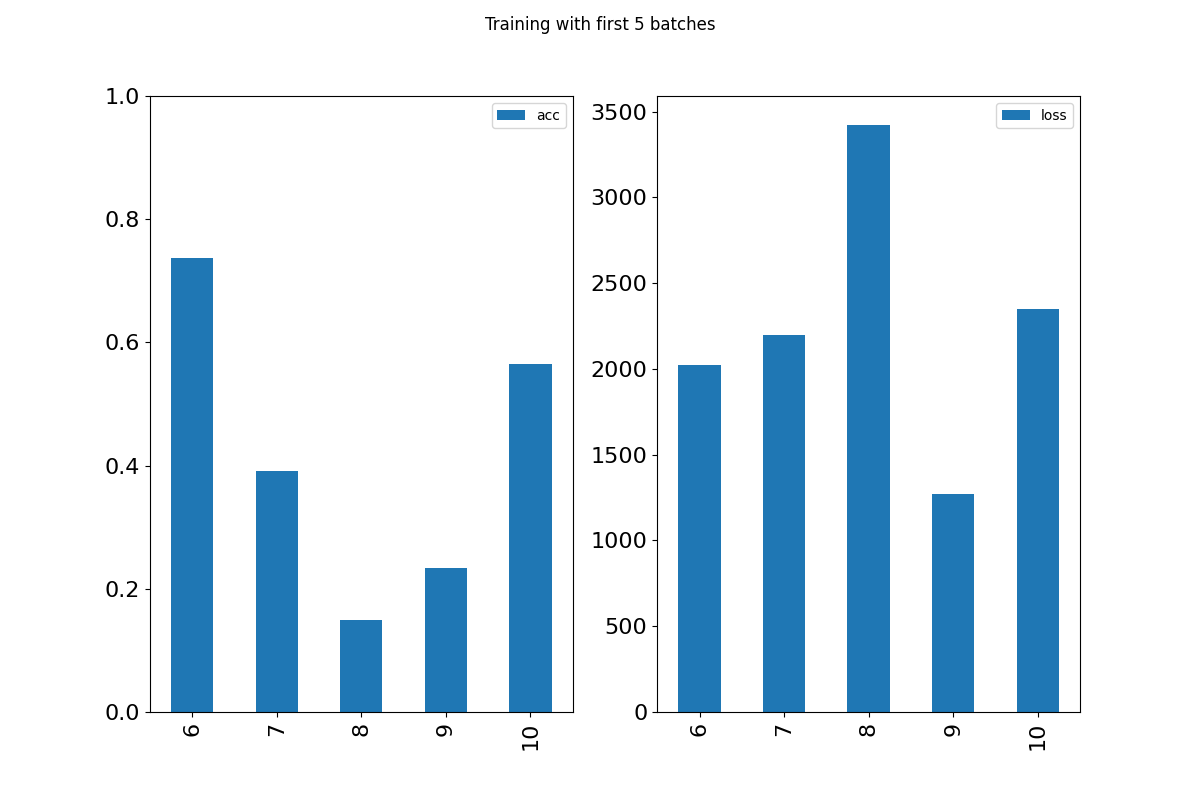
\includegraphics[width=0.45\linewidth]{../py_imgs/Step1_NBATCH_5_acc_loss}
	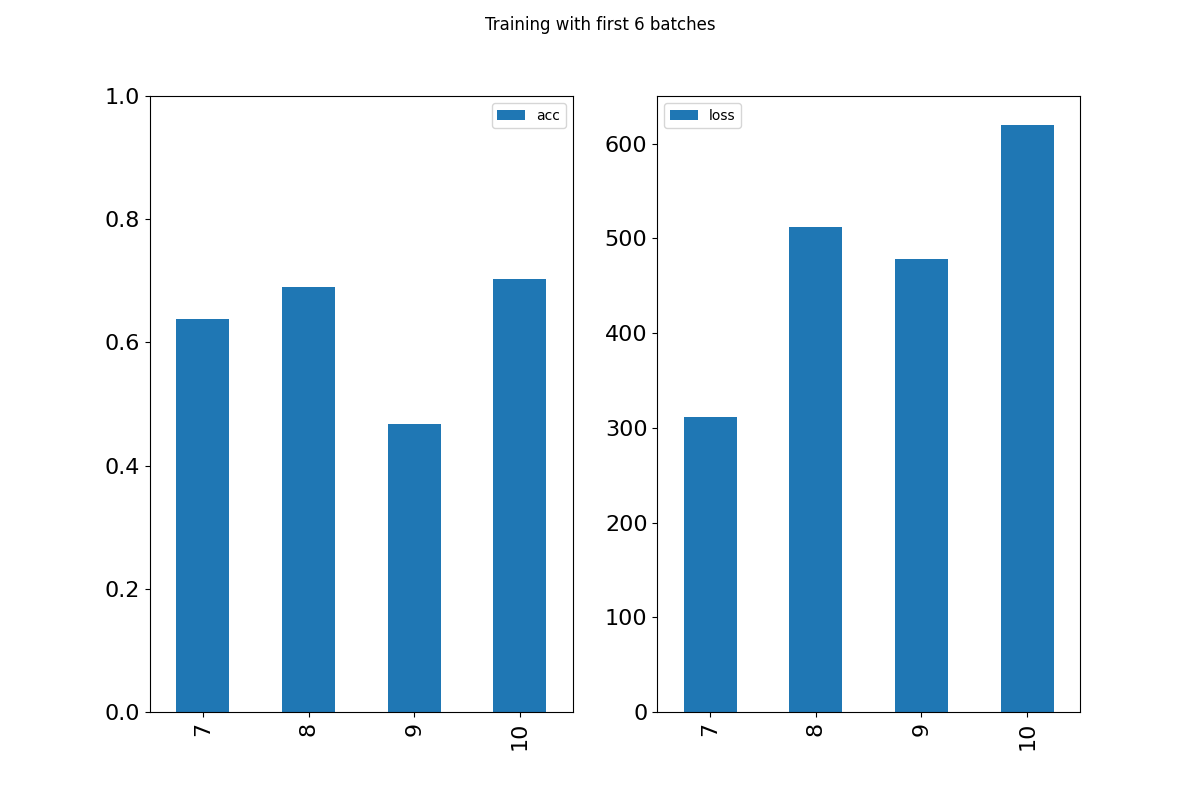
\includegraphics[width=0.45\linewidth]{../py_imgs/Step1_NBATCH_6_acc_loss}
	\caption[Evolución del drift con los resultados de validación]{Evolución del drift con los resultados de validación. Utilizando un numero N de lotes como entrenamiento, y calculando su accuracy y loss frente a los siguientes batchs de forma individual. }
	\label{fig:EvoModelSimpleBatch}
\end{figure}


Esto nos indica que la deriva es acumulativa, conforme mas nos alejamos de los meses de entrenamiento peor accuracy tiene el modelo.


Debemos mencionar que estos resultados se han obtenido utilizando los datos de los 16 sensores, que como ya se mencionó guardan una fuerte correlación. 


Esto podría hacer que el modelo no diera importancia al resto de variables, ya que siempre es necesario entrenar los modelos con variables independientes. La multicolinealidad reduce la precisión de los coeficientes de estimación, lo que debilitaría los modelos de regresión, y por tanto cualquier modelo basado en regresión: redes neuronales, random forest, etc.

Sin embargo, es posible que este efecto se vea compensado por la información añadida que sí que aporta, ya que el gas a una concentración dada pasaría de estar definido por 8 variables a 128.

Al utilizar RandomForest y LightGBM se han encontrado la misma evolución. Cabe destacar que LightGBM es increíblemente rápido para entrenar. 

\begin{figure}
	\centering
	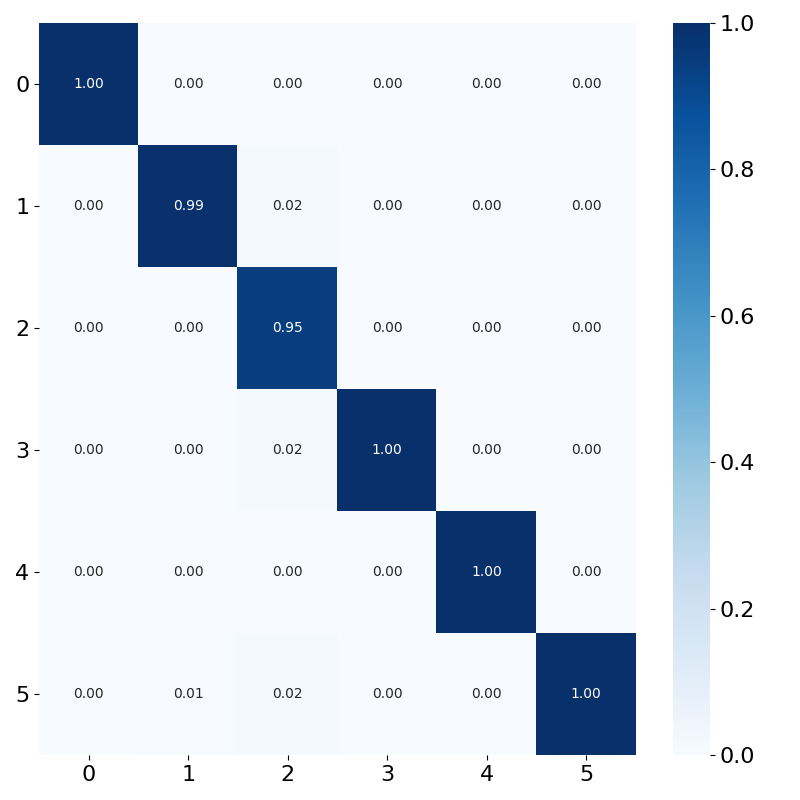
\includegraphics[width=0.6\linewidth]{../py_imgs/Setp4_conf_matrix_batch1to9}
	\caption{Matriz de confusión utlizando todos los datos disponibles de los batchs 1 a 9. Los datos de entramiento y datos de validacion se han divido al 70-30}
	\label{fig:setp4confmatrixbatch1to9}
\end{figure}

\begin{figure}
	\centering
	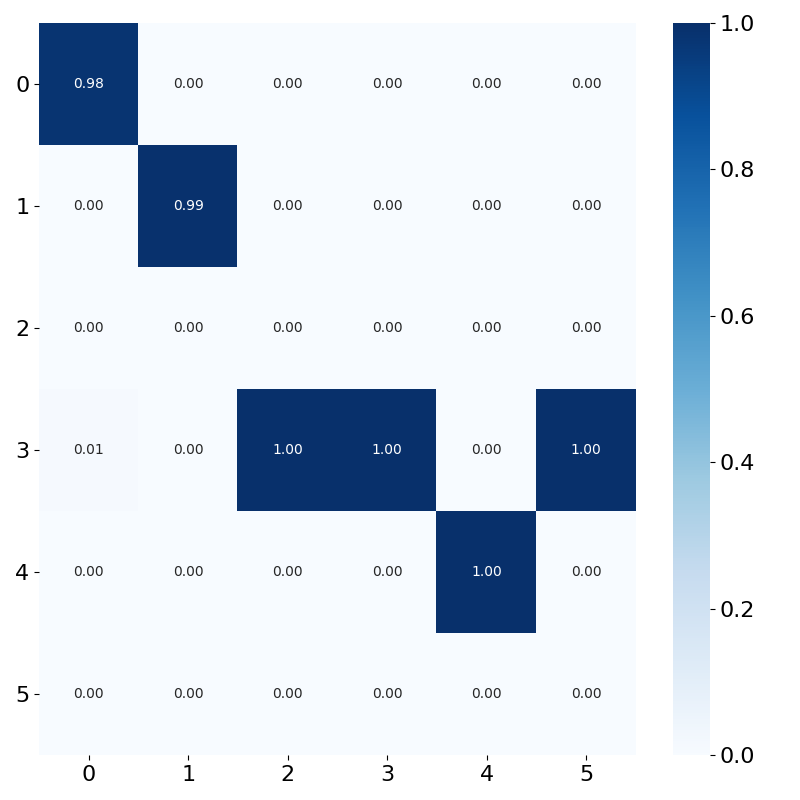
\includegraphics[width=0.6\linewidth]{../py_imgs/Setp4_conf_matrix_test_with_batch10}
	\caption{Matriz de confusión enfrentando el modelo a los datos nuevos proporcionados en le batch 10. El modelo sigue siendo preciso, pero no accurate, ya que confunde los gases.Podemos ver que 2 y 5 son catalogados como gas3. }
	\label{fig:setp4confmatrixbatch1to9}
\end{figure}


\subsection{Efecto del tipo de sensor}

Vamos a entrenar 4 modelos, uno utilizando las mediciones de cada tipo de sensor, y compararemos las matrices de confusión, para ver si hay sensores que no consiguen detectar un gas específico. Denominemos al tipo de sensor A,B,C y D.

\begin{figure}
	\centering
	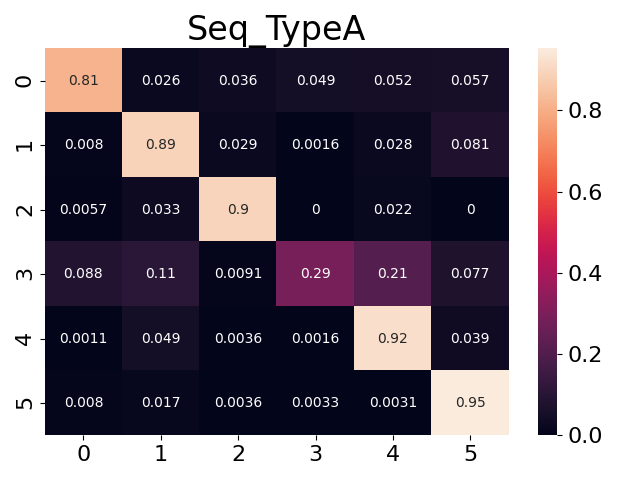
\includegraphics[width=0.45\linewidth]{../py_imgs/Conf_Seq_TypeA}
	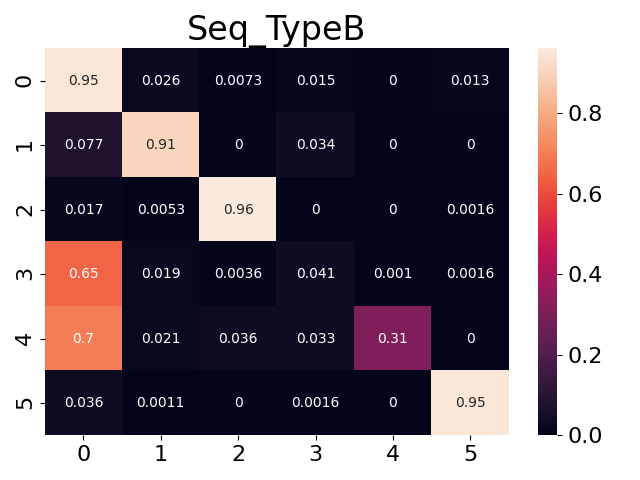
\includegraphics[width=0.45\linewidth]{../py_imgs/Conf_Seq_TypeB}
	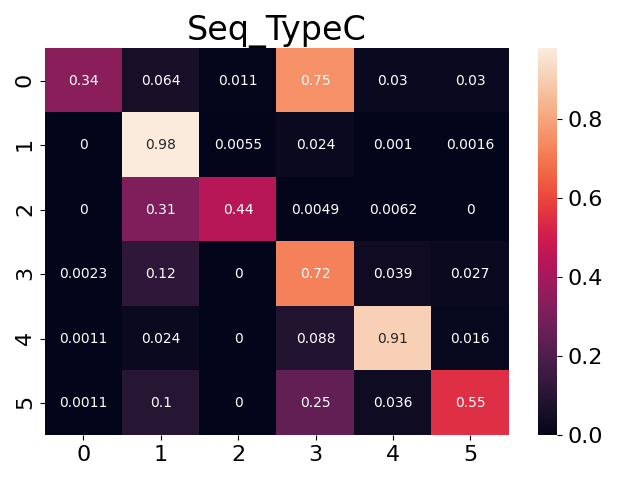
\includegraphics[width=0.45\linewidth]{../py_imgs/Conf_Seq_TypeC}
	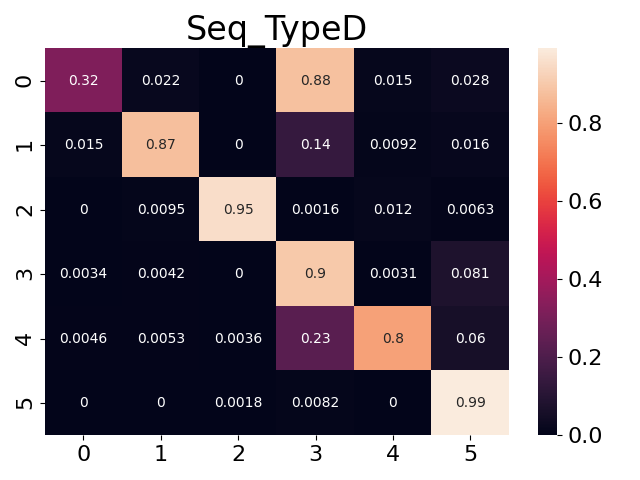
\includegraphics[width=0.45\linewidth]{../py_imgs/Conf_Seq_TypeD}
	\caption[Matrix de confusión para cada tipología de sensor]{ Matriz de confusión utilizando solo sensores tipo A en la img sup izq, solo sensores tipo B en la img sup drech y así sucesivamente. El sensor tipo A predice bastante bien todos los tipos de gases, los sensores B no consiguen detectar dos gases, y los tipo C y D fallan mucho al detectar un gas en concreto.   }
	\label{fig:confseqtypea}
\end{figure}

\begin{figure}
	\centering
	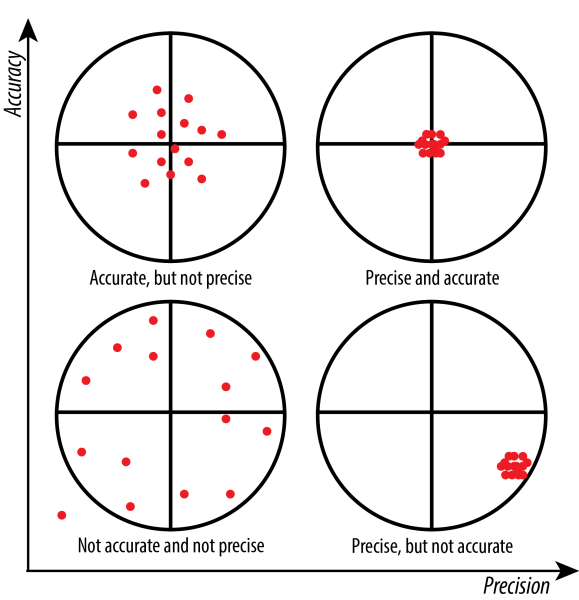
\includegraphics[width=0.7\linewidth]{../py_imgs/precsion_vs_accuracy}
	\caption[Accuracy y precision]{Es importante diferenciar entre accuracy y precision, ya que según de que forma fallen nuestros modelos, ya que podria aportarnos información sobre el problema al que nos enfrentamos.}
	\label{fig:precisionvsaccuracy}
\end{figure}

Las diferencias de sensibilidad entre cada sensor del mismo tipo influyen en sus predicciones. La efectividad de los modelos basados en cada sensor es peor que el modelo total. Pero cabe la posibilidad de que el modelo de 128 dimensiones esté desechando muchas dimensiones, no utilizando la información proporcionada por todos los sensores.

La Figura \ref{fig:confseqtypea} nos da mucha informacón sobre qué está ocurriendo , ya que el modelo de tipoB no es accuracy, pero sí precise, ya que los gases 3, y 4 los está clasificando como gas0. (ver Figura \ref{fig:precisionvsaccuracy})

Si utilizamos RandomForest o LightGBM, podemos representar los shap values, y ver cuales son las variables que más están influyendo en el resultado de la predicción. Los shap values para un modelo entrenado únicamente con un sensor son razonables, \ref{fig:step4lgbmonesensor}, pero si utilizamos las 128 componentes disponibles vemos que el modelo está desechando mucha información, Figura \ref{fig:step4lgbmall-data}

\begin{figure}
	\centering
	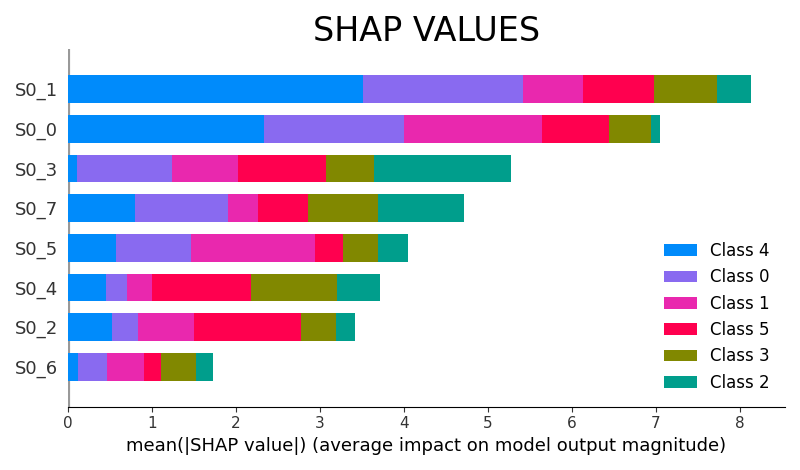
\includegraphics[width=0.7\linewidth]{../py_imgs/Step4_LGBM_one_sensor}
	\caption[Modelo LGBM-1sensor]{Modelo de LGBM para un sensor. Prácticamente todas las variables tienen influencia en la predicción. }
	\label{fig:step4lgbmonesensor}
\end{figure}

\begin{figure}
	\centering
	\includegraphics[width=0.7\linewidth]{"../py_imgs/Step4_LGBM_all data"}
	\caption[Modelo LGBM-6sensores]{Modelo de LGBM para todos los sensores. podemos obtervar que está tomando compoenntes aleatorias de cada sensor. De las 128 componentes, podriamos quedarnos únicamente con las 20 primeras y los resultados de la predicción serían similares. }
	\label{fig:step4lgbmall-data}
\end{figure}


\section{Algoritmos no supervisados}

Para este apartado se ha elegido dos algoritmos de clasificación no supervisada, KMeans clustering y TSNE. 

Para el algotirmo de KMeans clustering se ha realizado la Figura \ref{fig:step03color-for-each-cluster}. En la imagen drcha se puede apreciar cómo hay mediciones que están bien difenciadas del resto, mientras que hay un gran conjunto de ellas que el algoritmo no ha podido separarlas, ya que se trata de mediciones muy similares, pero sin embargo e trata de gases distintos. 
	
Esto pone de manifiesto la complejidad del problema, ya que si las señales para cada gas fueran suficientemente diferentes entre sí, el algoritmo de clustering no habria encontrado problema en diferenciarlas. 

\begin{figure}[h!]
	\centering
	\includegraphics[width=0.45\linewidth]{"../py_imgs/Step0_3_Color for each cluster_3d_All data"}
	\includegraphics[width=0.45\linewidth]{"../py_imgs/Step0_3_Color for each gas_3d_All data"}
	\caption[Resultados KMeans Clustering]{En ambas imagenes los puntos están distribuidos según los planos propuestos por PCA. En la imagen a la izq podemos ver los grupos propuestos por el algorimo de KMeans Clusteing, mientras que a la derecha se ha coloreado cada punto según a qué gas pertenece dicha medición. }
	\label{fig:step03color-for-each-cluster}
\end{figure}


Otro algoritmo de clasificación no supervisada, TSNE \emph{t-distributed stochastic neighbor embedding}, nos ha dado como resultado la Figura \ref{fig:step03tsnecolor-for-each-gas}, donde se ha coloreado cada punto en función del gas al que pertenece. Esta imagen pone de manifiesta cómo hay mediciones que a pesar de pertenecer a otros gases, son tan similares a otras que acaban en un clúster que no les correponde. 

\begin{figure}[h!]
	\centering
	\includegraphics[width=0.9\linewidth]{"../py_imgs/Step0_3_TSNE_3d_All data"}
	\caption[Resultados TSNE]{Resultados TSNE. Se han coloreado los  puntos según a qué gas pertenece. Se observa que no es capaz de separar los clusters de forma unívoca para cada medición.}
	\label{fig:step03tsnecolor-for-each-gas}
\end{figure}

Si reducimos la dificultad del problema, creando un dataset con las mediciones de un solo sensor, concentraciones por debajo de 100, y utilizando el primer batch, obtenemos los gráficos de las Figuras \ref{}

\begin{figure}[h!]
	\centering
	\includegraphics[width=0.45\linewidth]{"../py_imgs/Step0_3_Color for each gas_Batch1_Sensor1_Conc less 100ppmv"}
	\includegraphics[width=0.45\linewidth]{"../py_imgs/Step0_3_Color for each gas_3d_Batch1_Sensor1_Conc less 100ppmv"}
	\caption[Resultados PCA modelo simplificado]{Resultados PCA para los datos del batch 1, sensor1 y concentraciones por debajo de 100ppmv. Se han coloreado los  puntos según a qué gas pertenece. A la izq se ha reducido la dimensionalidad a 2d, y a la drecha a 3d. Los fases aparecen en clusters bien diferenciados}
	\label{fig:step03kmeans-reduced-color-for-each-gas}
\end{figure}

\begin{figure}[h!]
	\centering
	\includegraphics[width=0.45\linewidth]{"../py_imgs/Step0_3_Color for each gas_Batch1and10_Sensor1_Conc less 100ppmv"}
	\includegraphics[width=0.45\linewidth]{"../py_imgs/Step0_3_Color for each gas_3d_Batch1and10_Sensor1_Conc less 100ppmv"}
	\caption[Resultados PCA modelo batch 1 y 10]{Resultados PCA para los datos del batch 1 y 10, sensor1 y concentraciones por debajo de 100ppmv. Se han coloreado los  puntos según a qué gas pertenece. A la izq se ha reducido la dimensionalidad a 2d, y a la drecha a 3d. Los puntos que han aparecido con respecto a la imagen anterior no se han agrupado con el cluster del batch 10, si no que han generado una nueva rama, lo que nos indica que son lo suficiente diferentes como para estar agrupadas aparte.}
	\label{fig:step03kmeans-1-10-color-for-each-gas}
\end{figure}


	\clearpage

	



	\clearpage

	\chapter{Conclusiones y planes de mejora}

\epigraph{johnny... johnny... JOHNNYYY!! {\textit{Seymour Skinner \\ The Simpsons}}

\lipsum[3-6]
	\clearpage

	\chapter{Conclusiones}
\lipsum[3-6]

	\appendix
	\chapter{Código utilizado}

\section{Código Exploratory Data Analysis}
\lstinputlisting[label={lst:Step0}, caption={Realiza el analisi exploratorio de los datos disponibles}, language={Python}]{../python/Step0_EDA.py}

\section{Código Red neuronal secuencial}
\lstinputlisting[label={lst:SeqNeuralNet}, caption={Red neuronal secuencial}, language={Python}]{../python/SeqModel.py}

\lstinputlisting[label={lst:Step1}, caption={Red neuronal secuencial para clasificar gases}, language={Python}]{../python/Step1_NN.py}

\section{Código LGBM}
\lstinputlisting[label={lst:Step4}, caption={Red neuronal secuencial para clasificar gases}, language={Python}]{../python/Step4_LightGBM.py}

\section{Codigo Randonforest}
\lstinputlisting[label={lst:RF},caption={Clases para cargar datos en memoria}, language={Python}]{../python/RandomForestClasification.py}
\lstinputlisting[label={lst:RFmain},caption={Clases para cargar datos en memoria}, language={Python}]{../python/Step2_RF_for_all_sensors.py}

\section{Código aprendizaje no supervisado} 
\lstinputlisting[label={lst:Cluster},caption={Clases para cargar datos en memoria}, language={Python}]{../python/Step0_3_ClusteringSignals.py}

\section{Código Utilities}
\lstinputlisting[label={lst:LoadUciData},caption={Clases para cargar datos en memoria}, language={Python}]{../python/LoadUciData.py}

\lstinputlisting[label={lst:LoadSensorData},caption={Clases para cargar datos en memoria}, language={Python}]{../python/LoadSensorData.py}

\lstinputlisting[label={lst:FileUtils},caption={Clases para cargar datos en memoria}, language={Python}]{../python/FileUtils.py}


	\clearpage

	\printglossaries
	\renewcommand{\url}[1]{\href{#1}{link}}
	% Uncomment the following line to print the entire bibliography
	\nocite{*}
	\bibliographystyle{apacite}
	\bibliography{Bibliography/TFMbibliografia}
	%
\end{document}
%%%%%%%%%%%%%%%%%%%%%%%%%%%%%%%%%%%%%%
